\documentclass{article}

\usepackage{graphicx}
\usepackage{hyperref}
\usepackage{caption}
\usepackage{subcaption}
\usepackage{booktabs}
\usepackage{tabularx}
\usepackage{multirow}
\usepackage{textcomp}
\usepackage{amsmath}
\usepackage[vmargin=0.8in, hmargin=1.5in]{geometry}

% Title and author information
\title{Machine Learning and Pattern Recognition Project Report}
\author{Paolo Magliano s314867}

\begin{document}

\maketitle

\begin{abstract}
This report describes the work done on Machine Learning and Pattern Recognition project. The report follows the structure of course laboratories, which studies and analyses the dataset and the models:
\begin{itemize}
    \item Multivariate Gaussian Model
    \item Logistic Regression
    \item Support Vector Machines
    \item Gaussian Mixture Model
\end{itemize}
\end{abstract}

% \tableofcontents

\section{Lab 2: Dataset}
\label{sec:dataset}
The samples are computed by a feature extractor that summarizes high-level characteristics of a fingerprint image. The data is 6-dimensional and it consists of labeled samples corresponding to the genuine (True, label 1) class and the fake (False, label 0) class.

The dataset can be summarized by the image in Figures \ref{fig:dataset}. It shows the data distribution of features and their correlation with each other.

\begin{figure}[ht]
    \centering
    \begin{subfigure}[b]{0.3\textwidth}
        \centering
        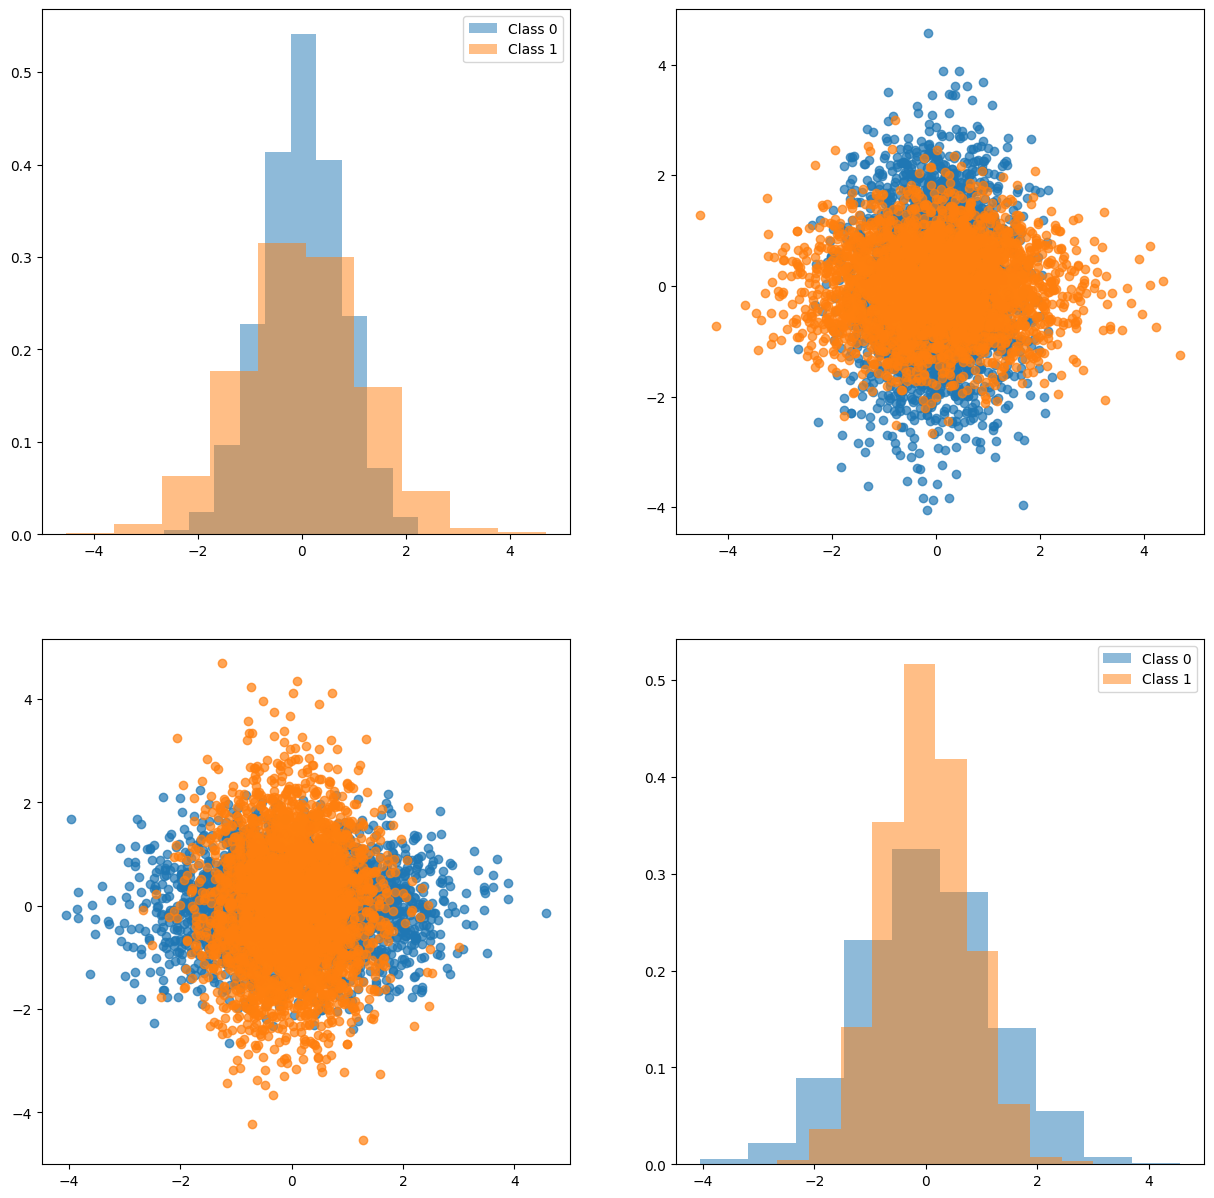
\includegraphics[width=\textwidth]{images/dataset_12.png}
        \caption{Features 1 and 2.}
    \end{subfigure}
    \hfill
    \begin{subfigure}[b]{0.3\textwidth}
        \centering
        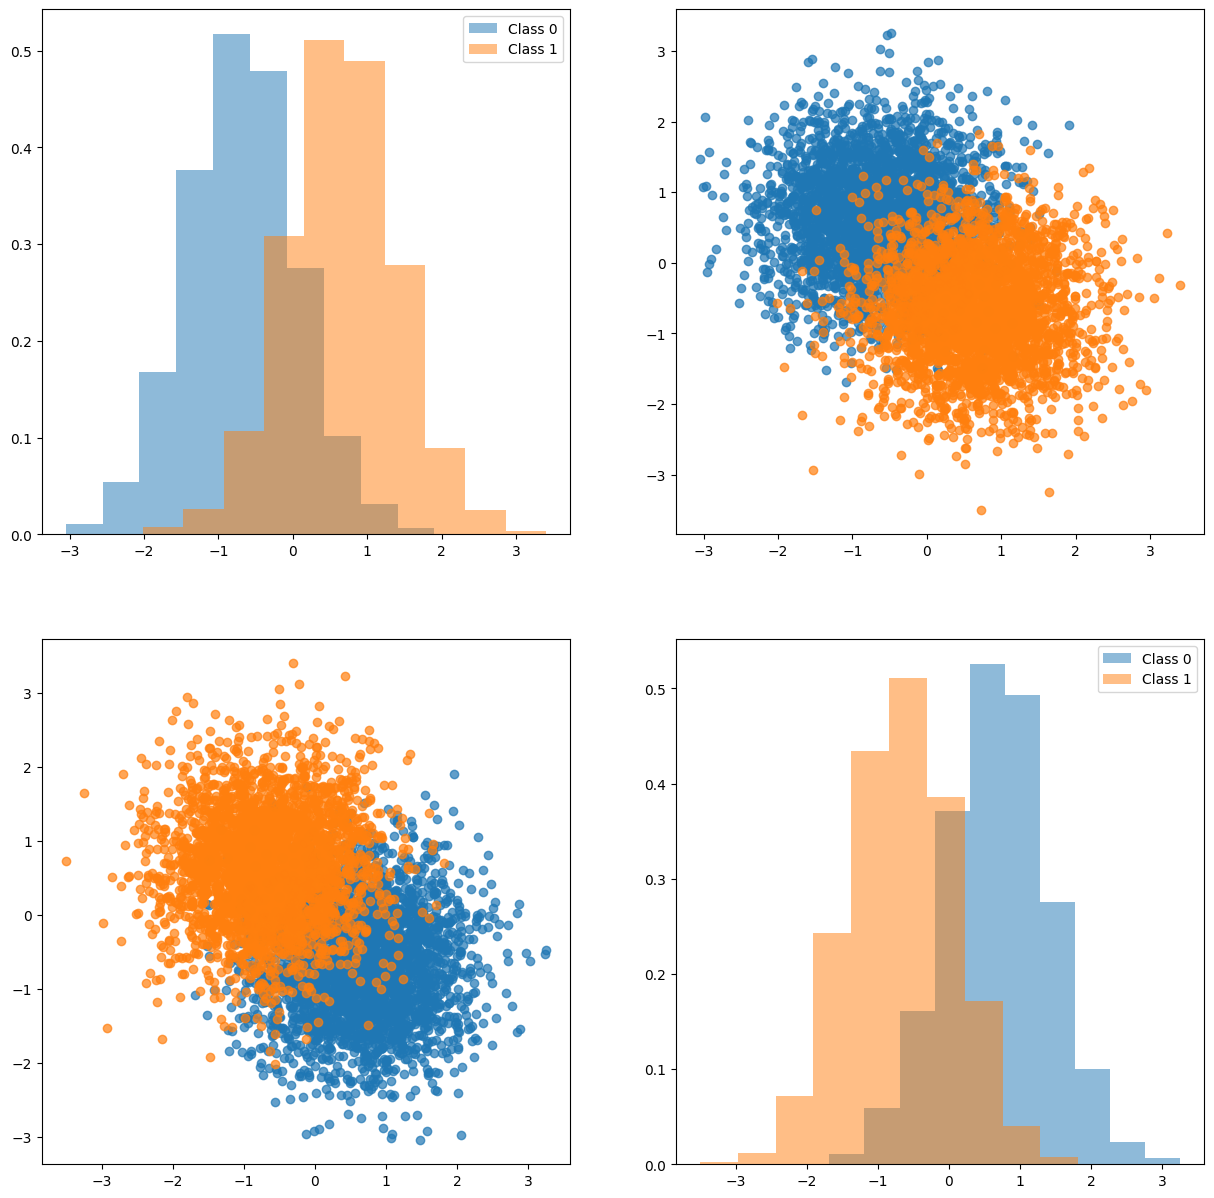
\includegraphics[width=\textwidth]{images/dataset_34.png}
        \caption{Features 3 and 4.}
    \end{subfigure}
    \hfill
    \begin{subfigure}[b]{0.3\textwidth}
        \centering
        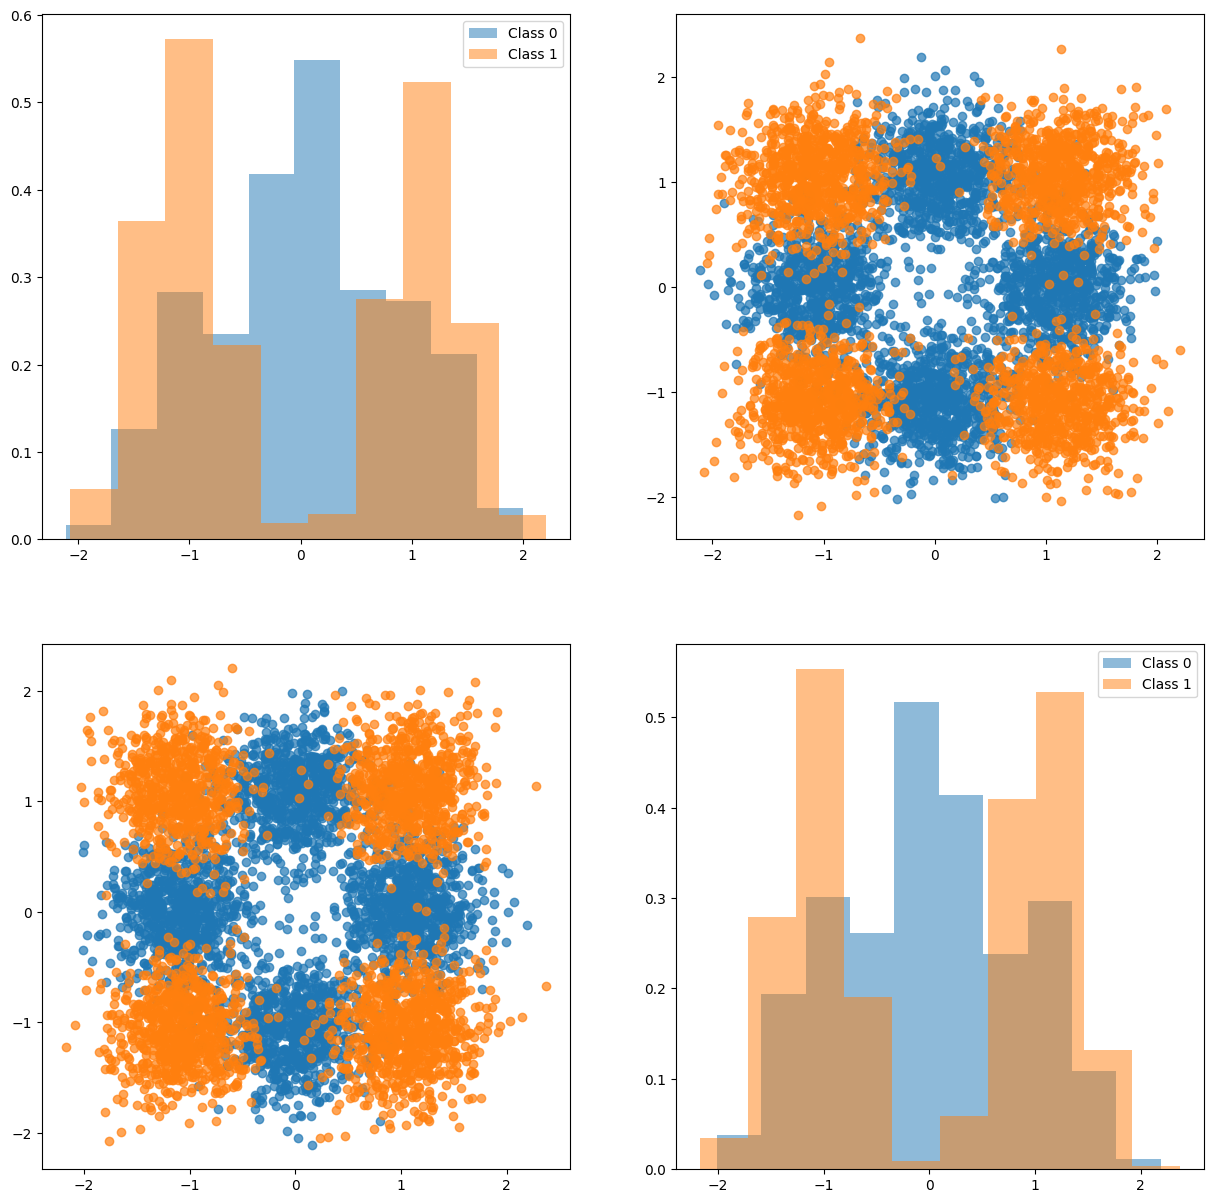
\includegraphics[width=\textwidth]{images/dataset_56.png}
        \caption{Features 5 and 6.}
    \end{subfigure}
    \caption{The figure shows histograms of the projected data on each feature. The scatter plot shows the correlation between the two features.}
    \label{fig:dataset}
\end{figure}

The first two features are mostly overlapping, so it is difficult to separate the two classes. The histograms show that they can be probably well approximated by a Gaussian density function. Further more means are very close to each other, but the variances are different. 

The third and fourth features are more separated, but still overlapping. Also these features can be approximated by a Gaussian density function but the means are different and variance very similar. These features are more useful in a classification task as they are more discriminative.

The last two features are the most discriminative, they can't be approximated by a simple unimodal Gaussian density function because they seems to be bimodal or trimodal. Thanks to this behavior they form 4 distinct clusters (two for each feature) that can be easily separated. They are probably the most useful features if the classifier is able to capture the complex structure.

\section{Lab 3: PCA and LDA}
\label{sec:pca_lda}

\subsection{Dimensionality Reduction}
Principal Component Analysis (PCA) is a dimensionality reduction technique that finds the directions of maximum variance in the data. It projects the data onto a lower-dimensional subspace while preserving as much variance as possible. The Figure \ref{fig:dataset_pca} shows the results of PCA on the dataset. The first principal component captures most of the variance and it separates decently the two classes. The other principal components overlap, so they are not very useful for classification.

\begin{figure}[ht]
    \centering
    \includegraphics[width=\textwidth]{images/dataset_pca.png}
    \caption{The figure shows the results of PCA on the dataset. The histograms show data distribution on each principal component. The top left one represents the first principal component, the bottom right is the last one. }
    \label{fig:dataset_pca}
\end{figure}

Linear Discriminant Analysis (LDA) is a supervised dimensionality reduction technique that finds the directions that maximize the separation between classes. The Figure \ref{fig:dataset_lda} shows the results of LDA on the dataset. Only one linear discriminant is found because the number of classes is 2. The linear discriminant separates the two classes partially. It is comparable to the first principal component of PCA.

\begin{figure}[ht]
    \centering
    \includegraphics[width=\textwidth]{images/dataset_lda.png}
    \caption{The figure shows the results of LDA on the dataset. The histogram shows data distribution on the only linear discriminant found.}
    \label{fig:dataset_lda}
\end{figure}

Both cases simplify the dataset as much that the well-distinctive cluster of the last two features is lost. So, the preprocessing techniques cloud be useful to speed up the computation but they could also lose important information. In very simple dataset ad this one, with only 6 dimensions, presumably the best choice is to use the original dataset.

\subsection{Classification}
The project analyses the performance of LDA method as a classifier. In order to get reliable results, the experiments' performance is evaluated with k-fold cross-validation with k equal to 10. It is also inspect the improvement of the classifier by using PCA as a preprocessing technique.

The Table \ref{tab:lda_performance} shows the performance results as error rate, Detection Cost Function (DCF) and Minimum DCF. The last one is useful to understand the gains of changing the threshold to optimal value.

\begin{table}[ht!]
    \centering
    \begin{tabularx}{\textwidth}{lXXX}
        \toprule
        \textbf{PCA} & \textbf{Error Rate (\%)} & \textbf{DCF} & \textbf{Min DCF} \\
        \midrule
        None   & 9.58 & 0.191 & 0.177 \\
        1 PC   & 9.68 & 0.193 & 0.179 \\
        2 PC   & 9.63 & 0.193 & 0.179 \\
        3 PC   & 9.43 & 0.189 & 0.177 \\
        4 PC   & 9.57 & 0.191 & 0.177 \\
        5 PC   & 9.58 & 0.192 & 0.177 \\
        6 PC   & 9.62 & 0.192 & 0.177 \\
        \bottomrule
    \end{tabularx}
    \caption{Performance metrics for LDA models with various dimensionality reduction techniques.}
    \label{tab:lda_performance}
\end{table}


As intuitively retrieved from PCA and LDA graphs, the capabilities of both methods are similar. In fact, the performance of the classifier is not improved by using PCA as a preprocessing technique. 

In general the performance are terrible considering the simplicity of the dataset. Further more the threshold selection is not optimal, so the performance could be improved by tuning it a little bit.

\section{Lab 4: Multivariate Gaussian density}
\label{sec:gaussian_density}
As preliminary step, the project analyses the correspondence between the features distribution and the Gaussian density function. This is helpful to understand the potential efficacy of model based on Gaussian density.
The figure \ref{fig:dataset_gaussian} shows the histograms of the dataset and the Gaussian density function that best fits the data.

\begin{figure}[ht]
    \centering
    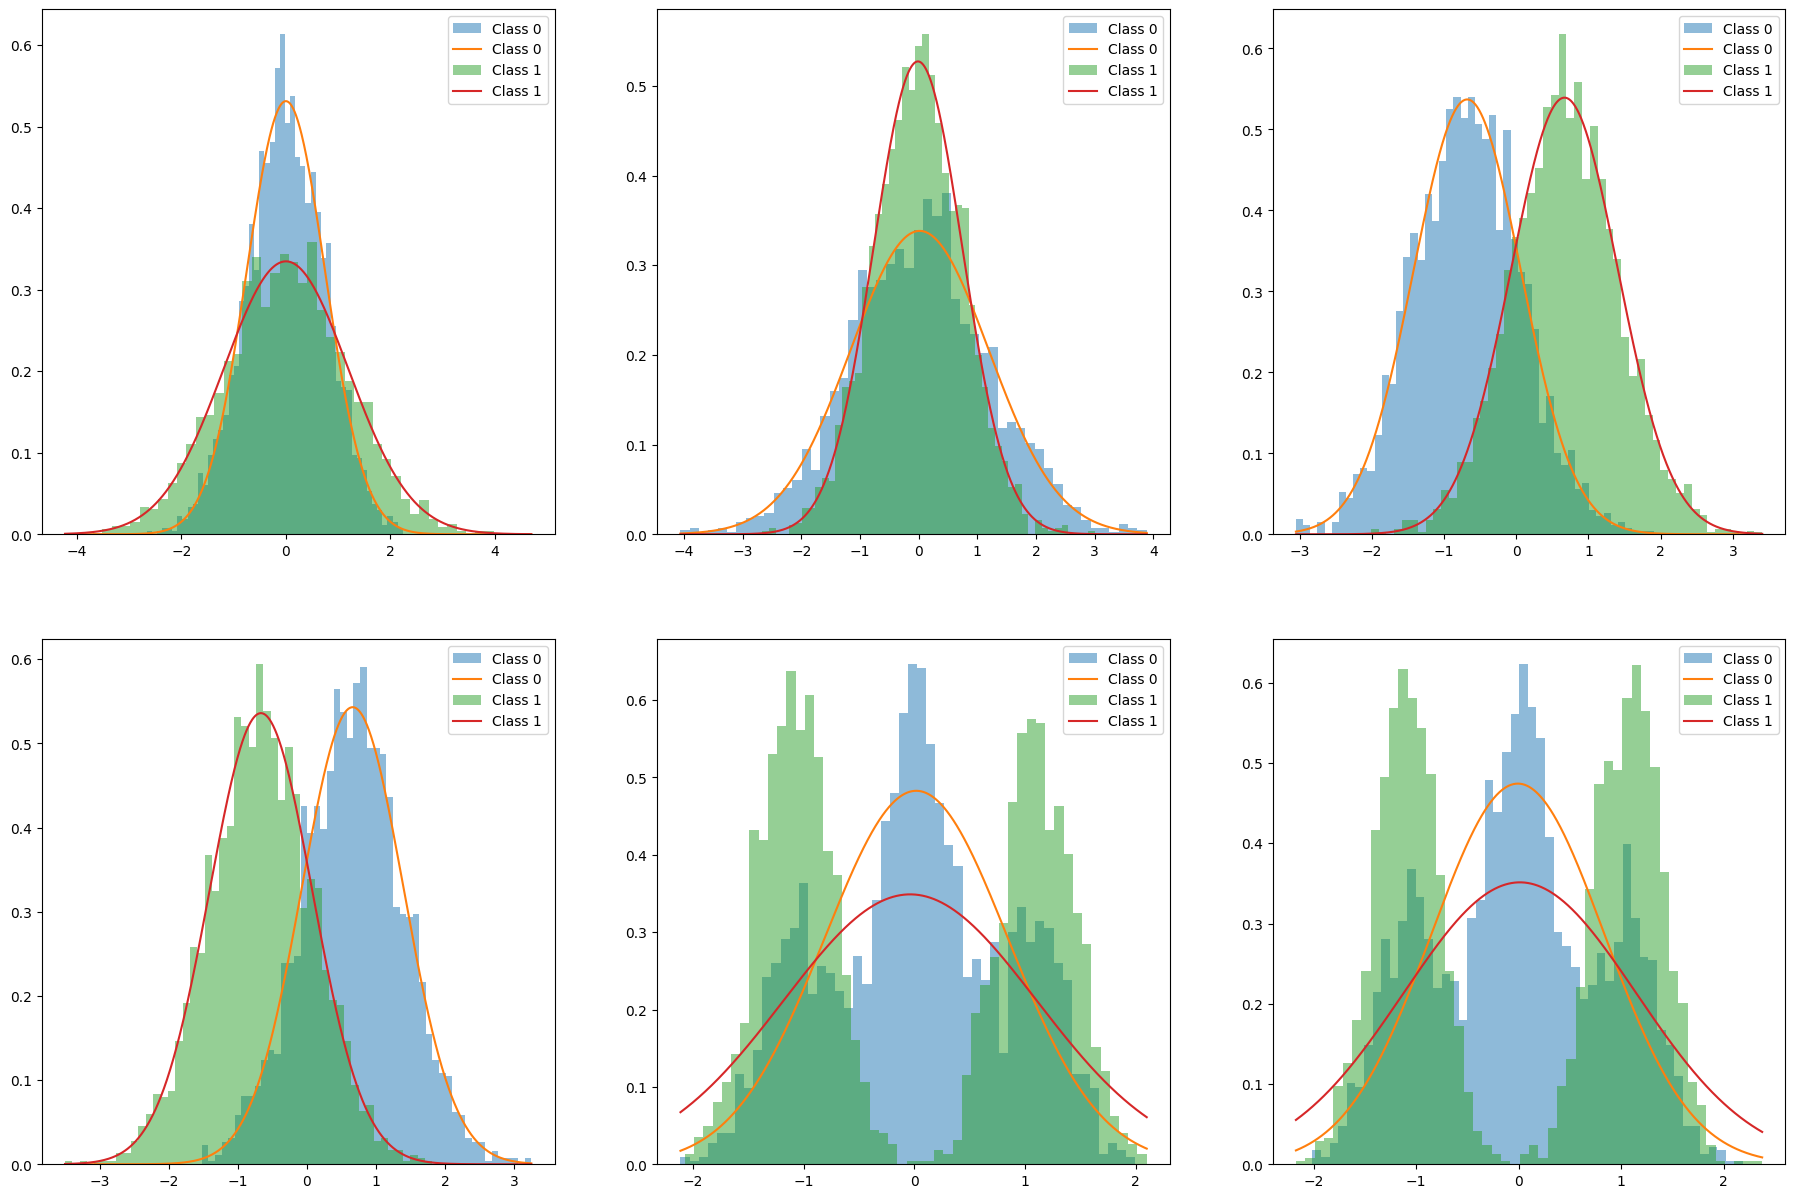
\includegraphics[width=\textwidth]{images/dataset_gaussian.png}
    \caption{The figure shows the histograms of the dataset and the Gaussian density function that best fits each feature.}
    \label{fig:dataset_gaussian}
\end{figure}

The results are consistent with the previous analysis. The first four features can be approximated by a unimodal Gaussian density function. Instead, the last two can not be well represented thanks to their multimodality.


\section{Lab 5: Multivariate Gaussian Model}

The project analyses the performance of Multivariate Gaussian (MVG) models with different covariance matrices: full, tied, and diagonal. The experiments are conducted with k-fold cross-validation with k equal to 10. The results are shown in Table \ref{tab:mvg_performance}.

\begin{table}[ht!]
    \centering
    \begin{tabularx}{\textwidth}{lXXX}
        \toprule
        \textbf{Model} & \textbf{Error Rate (\%)} & \textbf{DCF} & \textbf{Min DCF} \\
        \midrule
        MVG      & 7.45 & 0.148 & 0.133 \\
        TiedMVG  & 9.62 & 0.192 & 0.177 \\
        NaiveMVG & 7.48 & 0.149 & 0.132 \\
        \bottomrule
    \end{tabularx}
    \caption{Performance metrics for various MVG models without dimensionality reduction.}
    \label{tab:mvg_performance}
\end{table}

The results show that the tied MVG performs worse than the others. This is due to the fact that the covariance matrix change considerably along the features and so it can't be approximated by a single matrix. To visualize this better, the Figure \ref{fig:dataset_gaussian_tied} shows the estimated Gaussian density function for the tied MVG model.

\begin{figure}[ht]
    \centering
    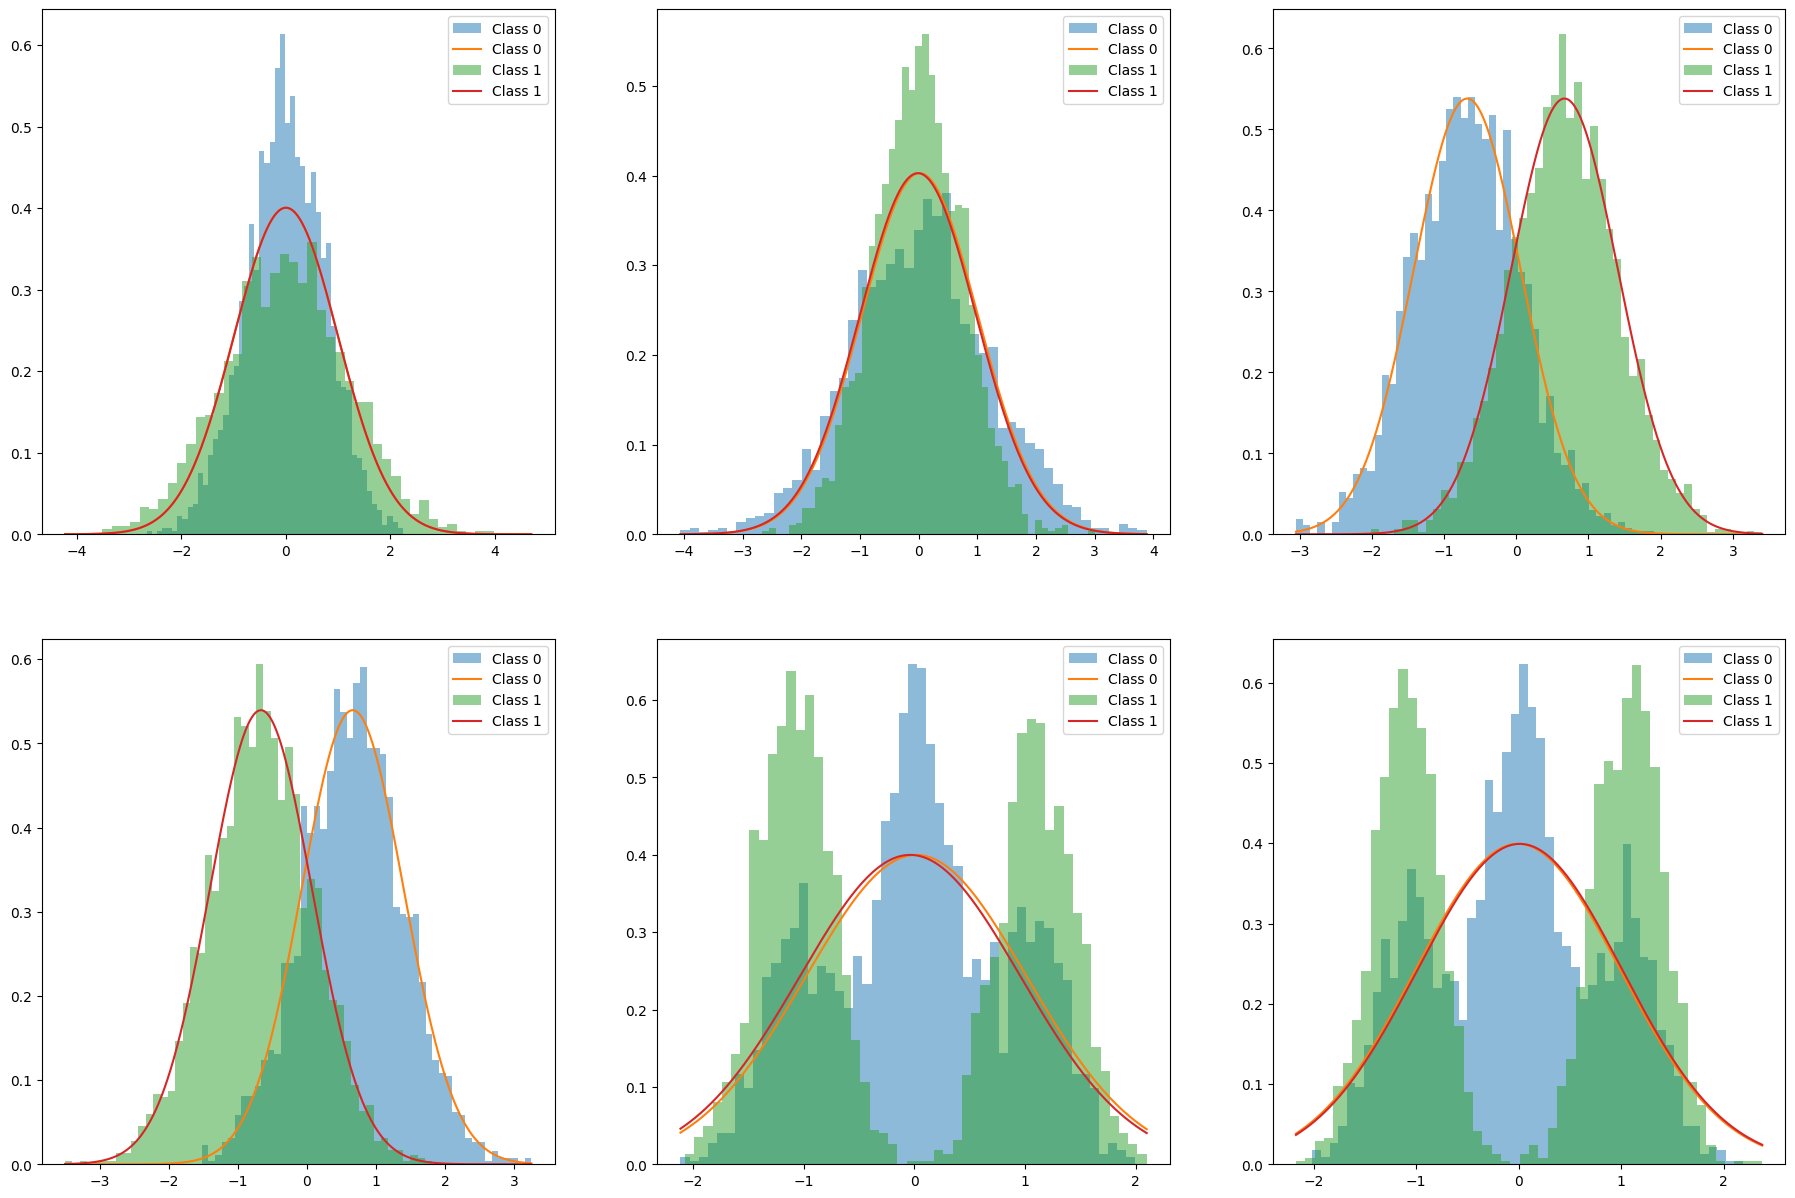
\includegraphics[width=\textwidth]{images/dataset_gaussian_tied.png}
    \caption{The figure shows the histograms of the dataset and the Gaussian density function with tied covariance matrix for each feature.}
    \label{fig:dataset_gaussian_tied}
\end{figure}

The graphs show that the tied MVG model can practically use only features 3 and 4 as discriminative ones. The other features are approximated with the same gaussian function fro both classes.

\subsection{Correlation Analysis}

In order to analyze further the performance of Naive MVG model respect to the full MVG model, the project computes the pearson correlation coefficient between the features for each class. The results are shown in Figure \ref{fig:dataset_person}. 
\begin{figure}[ht]
    \centering
    \begin{subfigure}[b]{0.45\textwidth}
        \centering
        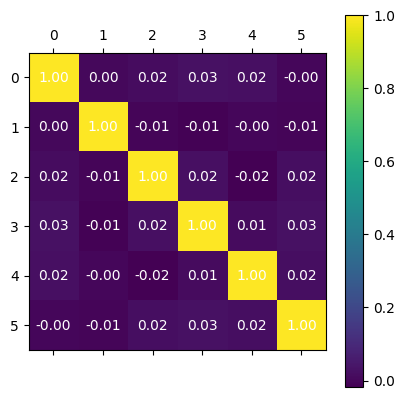
\includegraphics[width=\textwidth]{images/dataset_pearson_false.png}
        \caption{Class False.}
    \end{subfigure}
    \hfill
    \begin{subfigure}[b]{0.45\textwidth}
        \centering
        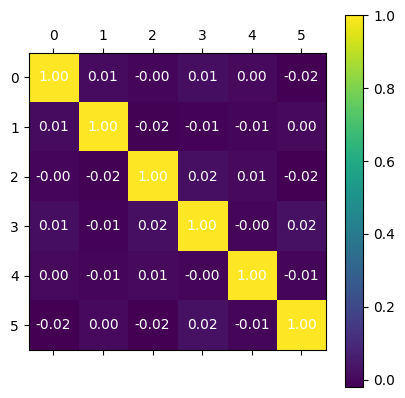
\includegraphics[width=\textwidth]{images/dataset_pearson_true.png}
        \caption{Class True.}
    \end{subfigure}
    \caption{The figure shows the Pearson correlation coefficient between the features for each class. Correlated features are close to 1 or -1.}
    \label{fig:dataset_person}
\end{figure}

The graphs show the reason why the Naive MVG model performs as well as the full MVG model. The features are not correlated at all, so the assumption of independence is not violated. 

\subsection{Assumption Analysis}

The Gaussian model assumes that features can be jointly modeled by Gaussian distributions. The good-ness of the model is therefore strongly affected by the accuracy of this assumption. As already discussed, the last two features do not satisfy this assumption. To analyze if indeed the last set of features negatively affects our classifier, we can try repeating the classification using only feature 1 to 4. The results are shown in Table \ref{tab:mvg_performance_4}.

\begin{table}[ht!]
    \centering
    \begin{tabularx}{\textwidth}{lXXX}
        \toprule
        \textbf{Model} & \textbf{Error Rate (\%)} & \textbf{DCF} & \textbf{Min DCF} \\
        \midrule
        MVG      & 8.35 & 0.167 & 0.149 \\
        TiedMVG  & 9.73 & 0.194 & 0.176 \\
        NaiveMVG & 8.35 & 0.167 & 0.149 \\
        \bottomrule
    \end{tabularx}
    \caption{Performance metrics for various MVG models with only the first 4 features.}
    \label{tab:mvg_performance_4}
\end{table}

For both MVG and Naive MVG models, the performance is slightly worse than the full dataset. This implies that the last two features are useful anyway, even if they are not well approximated by a Gaussian. 

\subsection{Mean and Variance of Features Analysis}

To further explore how means and variance of the features affect the performance of different approaches, the project repeats the classification using only features 1 and 2 and then only features 3 and 4. This is done because features 1 and 2 means are similar but variances are not, whereas for features 3 and 4 the two classes mainly differ for the feature mean, but show similar variance. The results are shown in Table \ref{tab:mvg_performance_12} and Table \ref{tab:mvg_performance_34}.

\begin{table}[ht!]
    \centering
    \begin{tabularx}{\textwidth}{lXXX}
        \toprule
        \textbf{Model} & \textbf{Error Rate (\%)} & \textbf{DCF} & \textbf{Min DCF} \\
        \midrule
        MVG      & 36.83 & 0.737 & 0.711 \\
        TiedMVG  & 49.55 & 0.99  & 0.887 \\
        NaiveMVG & 36.80 & 0.737 & 0.711 \\
        \bottomrule
    \end{tabularx}
    \caption{Performance metrics for various MVG models with only the first 2 features.}
    \label{tab:mvg_performance_12}
\end{table}

\begin{table}[ht!]
    \centering
    \begin{tabularx}{\textwidth}{lXXX}
        \toprule
        \textbf{Model} & \textbf{Error Rate (\%)} & \textbf{DCF} & \textbf{Min DCF} \\
        \midrule
        MVG      & 9.67 & 0.193 & 0.176 \\
        TiedMVG  & 9.68 & 0.194 & 0.177 \\
        NaiveMVG & 9.68 & 0.194 & 0.177 \\
        \bottomrule
    \end{tabularx}
    \caption{Performance metrics for various MVG models with only the 3 and 4 features.}
    \label{tab:mvg_performance_34}
\end{table}

Lets first analyze the generale performance between the two cases. The performance of the first two features is terrible, this is due to the fact that the two classes are not separable at all and this shows how important is the mean of class distribution. Instead, the performance of features 3 and 4 is very good, this is due to the fact that the two classes mean are very different and this remark how much these features are discriminative.

More over, in the first case Tied MVG model performs even worse because the features' variances are unsimilar. Instead in the second case, the performances are the same for all models because the features' variances are pretty the same.

\subsection{Dimensionality reduction}
Finally the project investigates the performance of MVG models with PCA as a preprocessing technique. The results are shown in Table \ref{tab:mvg_performance_pca}.

\begin{table}[ht]
    \centering
    \begin{tabularx}{\textwidth}{ll*{6}{X}}
        \toprule
        \textbf{Model} & \textbf{Metrics} & \textbf{PCA 1} & \textbf{PCA 2} & \textbf{PCA 3} & \textbf{PCA 4} & \textbf{PCA 5} & \textbf{PCA 6} \\
        \midrule
        \multirow{3}{*}{MVG} & Error & 9.7\% & 9.23\% & 8.78\% & 8.33\% & 7.38\% & 7.45\% \\
                              & DCF & 0.194 & 0.185 & 0.175 & 0.166 & 0.147 & 0.148 \\
                              & Min DCF & 0.179 & 0.173 & 0.161 & 0.151 & 0.133 & 0.133 \\
        \midrule
        \multirow{3}{*}{TiedMVG} & Error & 9.68\% & 9.63\% & 9.45\% & 9.58\% & 9.57\% & 9.62\% \\
                                 & DCF & 0.193 & 0.193 & 0.189 & 0.191 & 0.191 & 0.192 \\
                                 & Min DCF & 0.179 & 0.177 & 0.177 & 0.177 & 0.177 & 0.177 \\
        \midrule
        \multirow{3}{*}{NaiveMVG} & Error & 9.7\% & 9.32\% & 9.3\% & 9.02\% & 8.58\% & 8.6\% \\
                                  & DCF & 0.194 & 0.186 & 0.186 & 0.18 & 0.172 & 0.172 \\
                                  & Min DCF & 0.179 & 0.174 & 0.166 & 0.162 & 0.158 & 0.158 \\
        \bottomrule
    \end{tabularx}
    \caption{Performance metrics for various MVG models with PCA as a preprocessing technique.}
    \label{tab:mvg_performance_pca}
\end{table}


The results confirm the hypothesis done in Dimensionality Reduction section. The performance of the classifier is not improved by using PCA as a preprocessing technique due to the lostness of the information. Indeed the best results are obtained with higher number of principal components. Tied MVG model is the only one that performs the same with and without PCA, this is due to PCA that provides features with similar variances.

\section{Lab 7: Model Evaluation}
\label{sec:model_evaluation}
The project proposes various metrics and tools to evaluate the performance of the models. The Detection Cost Function (DCF) is a metric that combines the error rate and the cost of false alarms and misses. The Minimum DCF is the DCF value at the optimal threshold. 

\subsection{Different Application}
In this section the project investigates the performance of the models in different application setups where the prior, the cost of false positives and the cost of false negatives are different. Specifically:
\begin{itemize}
    \item ($\pi_{\text{T}}, C_{\text{FP}}, C_{\text{FN}}$) = (0.5, 1, 1)
    \item ($\pi_{\text{T}}, C_{\text{FP}}, C_{\text{FN}}$) = (0.1, 1, 1)
    \item ($\pi_{\text{T}}, C_{\text{FP}}, C_{\text{FN}}$) = (0.9, 1, 1)
    \item ($\pi_{\text{T}}, C_{\text{FP}}, C_{\text{FN}}$) = (0.5, 1, 9)
    \item ($\pi_{\text{T}}, C_{\text{FP}}, C_{\text{FN}}$) = (0.5, 9, 1)
\end{itemize}
The image \ref{fig:confusion_matrix} shows the confusion matrix for the different application setups for the MVG model. 

\begin{figure}[ht]
    \centering
    \begin{subfigure}[b]{0.18\textwidth}
        \centering
        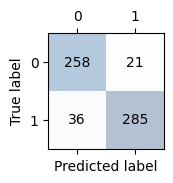
\includegraphics[width=\textwidth]{images/confusion_matrix_5_1_1.png}
        \caption{(0.5, 1, 1).}
    \end{subfigure}
    \hfill
    \begin{subfigure}[b]{0.18\textwidth}
        \centering
        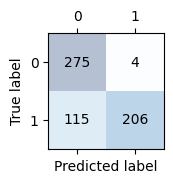
\includegraphics[width=\textwidth]{images/confusion_matrix_1_1_1.png}
        \caption{(0.1, 1, 1).}
    \end{subfigure}
    \hfill
    \begin{subfigure}[b]{0.18\textwidth}
        \centering
        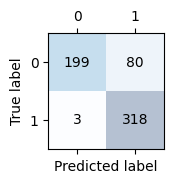
\includegraphics[width=\textwidth]{images/confusion_matrix_9_1_1.png}
        \caption{(0.9, 1, 1).}
    \end{subfigure}
    \hfill
    \begin{subfigure}[b]{0.18\textwidth}
        \centering
        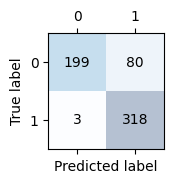
\includegraphics[width=\textwidth]{images/confusion_matrix_5_1_9.png}
        \caption{(0.5, 1, 9).}
    \end{subfigure}
    \hfill
    \begin{subfigure}[b]{0.18\textwidth}
        \centering
        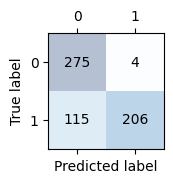
\includegraphics[width=\textwidth]{images/confusion_matrix_5_9_1.png}
        \caption{(0.5, 9, 1).}
    \end{subfigure}
    \caption{The figure shows the confusion matrix for the different application setups for the MVG model.}
    \label{fig:confusion_matrix}
\end{figure}

The confusion matrixes emphasize how the model choices depend on the prior and the cost of false positives and false negatives. For example, in the case (0.1, 1, 1) the model is biased towards the negative class, so the false negatives are very low. Instead, in the case (0.9, 1, 1) the model is biased towards the positive class, so the false positives are very low.

\subsection{Application Evaluation}
The project evaluates the performance of the models in the different application setups:
\begin{itemize}
    \item ($\pi_{\text{T}}, C_{\text{FP}}, C_{\text{FN}}$) = (0.5, 1, 1)
    \item ($\pi_{\text{T}}, C_{\text{FP}}, C_{\text{FN}}$) = (0.1, 1, 1)
    \item ($\pi_{\text{T}}, C_{\text{FP}}, C_{\text{FN}}$) = (0.9, 1, 1)
\end{itemize}
The results for (0.5, 1, 1) are already presented in Table \ref{tab:mvg_performance} and Table \ref{tab:mvg_performance_pca}. The results for the other two setups are shown in Table \ref{tab:mvg_performance_1_1_1}. and Table \ref{tab:mvg_performance_9_1_1}.

\begin{table}[ht]
    \centering
    \begin{tabularx}{\textwidth}{ll*{7}{X}}
        \toprule
        \textbf{Model} & \textbf{Metrics} & \textbf{None} & \textbf{1 PC} & \textbf{2 PC} & \textbf{3 PC} & \textbf{4 PC} & \textbf{5 PC} & \textbf{6 PC} \\
        \midrule
        \multirow{3}{*}{MVG} & Error & 13.68\% & 17.77\% & 16.82\% & 16.12\% & 15.15\% & 13.72\% & 13.68\% \\
                              & DCF & 0.37 & 0.481 & 0.457 & 0.433 & 0.419 & 0.378 & 0.37 \\
                              & Min DCF & 0.308 & 0.413 & 0.409 & 0.381 & 0.355 & 0.312 & 0.308 \\
        \midrule
        \multirow{3}{*}{TiedMVG} & Error & 17.42\% & 17.85\% & 17.55\% & 17.5\% & 17.4\% & 17.42\% & 17.42\% \\
                                 & DCF & 0.471 & 0.483 & 0.474 & 0.471 & 0.472 & 0.475 & 0.471 \\
                                 & Min DCF & 0.408 & 0.413 & 0.408 & 0.402 & 0.408 & 0.409 & 0.408 \\
        \midrule
        \multirow{3}{*}{NaiveMVG} & Error & 13.97\% & 17.77\% & 16.98\% & 16.3\% & 15.9\% & 15.42\% & 15.38\% \\
                                  & DCF & 0.373 & 0.481 & 0.466 & 0.439 & 0.431 & 0.41 & 0.409 \\
                                  & Min DCF & 0.31 & 0.413 & 0.41 & 0.393 & 0.369 & 0.363 & 0.362 \\
        \bottomrule
    \end{tabularx}
    \caption{Performance metrics for various MVG models with (0.1, 1, 1) application setup.}
    \label{tab:mvg_performance_1_1_1}
\end{table}

\begin{table}[ht]
    \centering
    \begin{tabularx}{\textwidth}{ll*{7}{X}}
        \toprule
        \textbf{Model} & \textbf{Metrics} & \textbf{None} & \textbf{1 PC} & \textbf{2 PC} & \textbf{3 PC} & \textbf{4 PC} & \textbf{5 PC} & \textbf{6 PC} \\
        \midrule
        \multirow{3}{*}{MVG} & Error & 14.05\% & 17.6\% & 16.25\% & 15.8\% & 14.87\% & 14.03\% & 14.05\% \\
                              & DCF & 0.367 & 0.464 & 0.45 & 0.439 & 0.399 & 0.364 & 0.367 \\
                              & Min DCF & 0.319 & 0.426 & 0.404 & 0.381 & 0.366 & 0.323 & 0.319 \\
        \midrule
        \multirow{3}{*}{TiedMVG} & Error & 17.05\% & 17.5\% & 17.4\% & 17.2\% & 17.13\% & 17.03\% & 17.05\% \\
                                 & DCF & 0.46 & 0.467 & 0.468 & 0.461 & 0.463 & 0.458 & 0.46 \\
                                 & Min DCF & 0.423 & 0.426 & 0.426 & 0.417 & 0.423 & 0.425 & 0.423 \\
        \midrule
        \multirow{3}{*}{NaiveMVG} & Error & 14.15\% & 17.6\% & 16.47\% & 16.05\% & 15.9\% & 15.57\% & 15.57\% \\
                                  & DCF & 0.364 & 0.464 & 0.451 & 0.439 & 0.433 & 0.411 & 0.411 \\
                                  & Min DCF & 0.32 & 0.426 & 0.403 & 0.397 & 0.384 & 0.359 & 0.36 \\
        \bottomrule
    \end{tabularx}
    \caption{Performance metrics for various MVG models with (0.9, 1, 1) application setup.}
    \label{tab:mvg_performance_9_1_1}
\end{table}

The results show that the performance of the models is strongly affected by the application setup and all the models suffer of big miscalibration error. Over all setups MVG model with full covariance matrix performs better than the others. As can be seen from min DCF values, all models can improve their performance by changing the threshold, despite they will never reach the value of (0.5, 1, 1) setup. The only setup well calibrated is (0.5, 1, 1) because the dataset is almost balanced according to the prior.

\subsection{Bayes Error Plot}
The project proposes a Bayes error plot to visualize the performance of the best MVG models: with PCA 6 for (0.1, 1, 1) application setup. The plot in Figure \ref{fig:mvg_bayes_error} compare the actual DCF and the min DCF for different application priors, understanding how well the model behaves in different scenarios.

\begin{figure}[ht]
    \centering
    \begin{subfigure}[b]{0.3\textwidth}
        \centering
        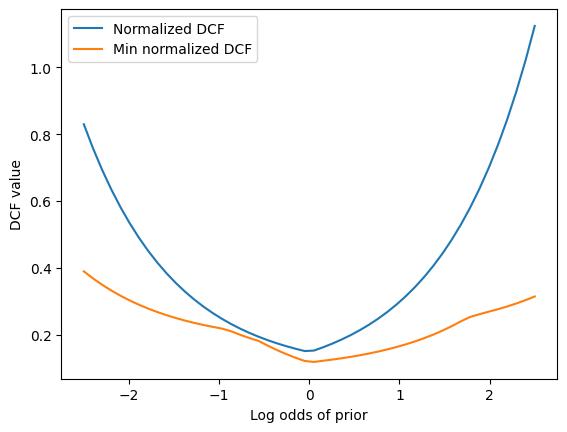
\includegraphics[width=\textwidth]{images/mvg_bayes_error.png}
        \caption{MVG model.}
    \end{subfigure}
    \hfill
    \begin{subfigure}[b]{0.3\textwidth}
        \centering
        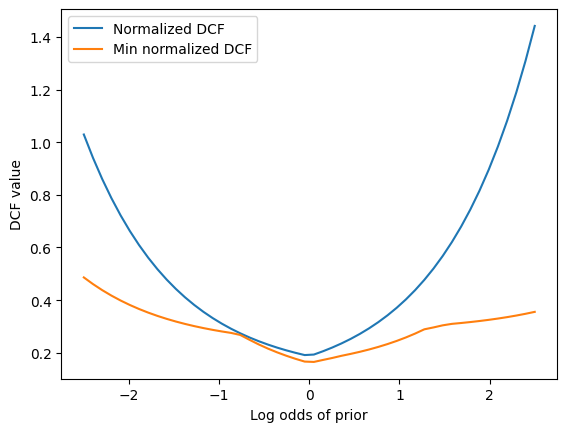
\includegraphics[width=\textwidth]{images/mvg_bayes_error_tied.png}
        \caption{TiedMVG model.}
    \end{subfigure}
    \hfill
    \begin{subfigure}[b]{0.3\textwidth}
        \centering
        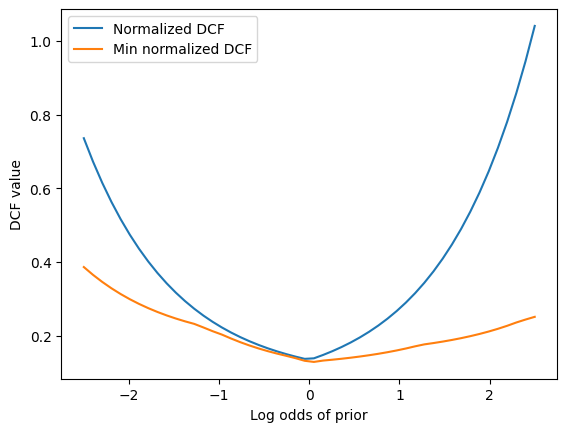
\includegraphics[width=\textwidth]{images/mvg_bayes_error_naive.png}
        \caption{NaiveMVG model.}
    \end{subfigure}
    \caption{The figure shows the Bayes error plot for the MVG models with PCA 6 for (0.1, 1, 1) application setup.}
    \label{fig:mvg_bayes_error}
\end{figure}

The Bayes error plot confirm the previous hypothesis on miscalibrated models. In fact, the actual DCF is often far from the min DCF and only in few cases the values are close to each other. 

At the end of the experiments the best model for application (0.1, 1, 1) is the MVG model with PCA 6 and min DCF equal to 0.308. The actual model is still a bit miscalibrated but not too much.

\section{Lab 8: Logistic Regression}
\label{sec:logistic_regression}
Logistic Regression (LR) is a classification model that estimates the probability of a binary outcome. The project explore the performance of both linear and quadratic LR models. The experiments are conducted with k-fold cross-validation with k equal to 10. 

\subsection{Regularization}
The project firstly investigates the performance of Logistic Regression (LR) model as it varies the regularization parameter $\lambda$. The Figure \ref{fig:lr_lambda} shows DCF and min DCF for different values of $\lambda$ evaluated with application setup (0.1, 1, 1).

\begin{figure}[ht]
    \centering
    \begin{subfigure}[b]{0.45\textwidth}
        \centering
        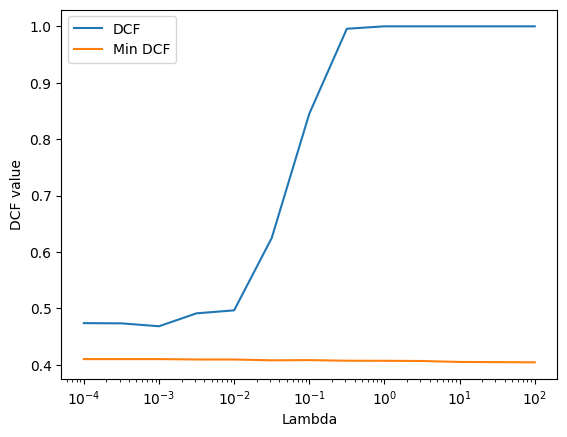
\includegraphics[width=\textwidth]{images/lr_lambda.png}
        \caption{All dataset}
        \label{fig:lr_lambda}
    \end{subfigure}
    \hfill
    \begin{subfigure}[b]{0.45\textwidth}
        \centering
        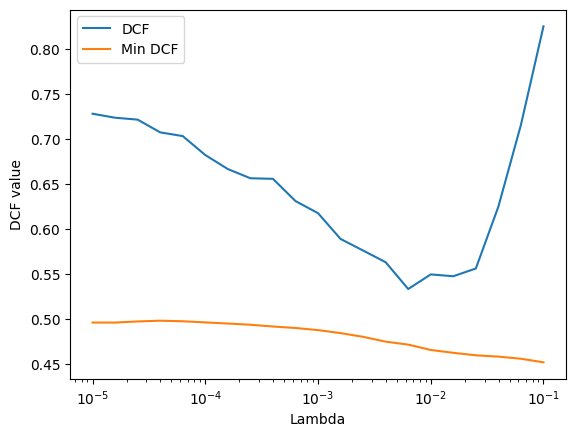
\includegraphics[width=\textwidth]{images/lr_lambda_100.png}
        \caption{$\frac{1}{100}$ dataset}
        \label{fig:lr_lambda_100}
    \end{subfigure}
    \caption{The figure shows the performance of LR models with different $\lambda$.}
\end{figure}

Since we have a large number of samples, regularization seems ineffective, and actually degrades actual DCF since the regularized models tend to lose the probabilistic interpretation of the scores. To better understand the role of regularization, the project analyses the results that we would obtain if we had fewer training samples. So, it repeats the previous analysis, but keep only 1 out of 100 model training sample and the results are shown in Figure \ref{fig:lr_lambda_100}.

The results show that regularization is useful when the number of samples is small. In fact, there is a range of values where the actual DCF decreases proportionally with increasing values of $\lambda$. In both cases, there is point (around 0.01) where higher value of $\lambda$ degrades drastically the performance of the model because it underfits too much the data. But before this point, the regularization is useful to avoid overfitting, in particular when the number of samples is small.

Further analysis are done using prior-weighted models to understand the difference respect to the standard one. The results are shown in Figure \ref{fig:lr_lambda_prior} and Figure \ref{fig:lr_lambda_100_prior}.

\begin{figure}[ht]
    \centering
    \begin{subfigure}[b]{0.45\textwidth}
        \centering
        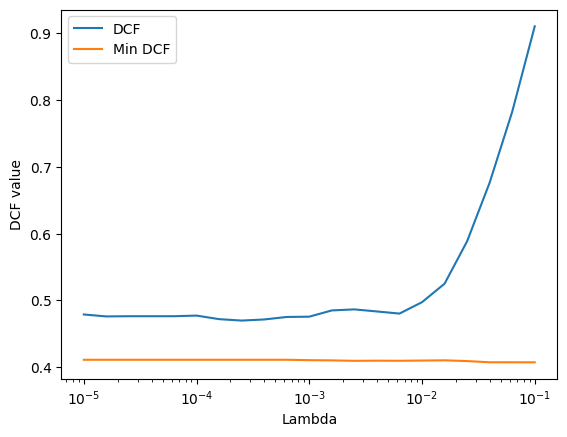
\includegraphics[width=\textwidth]{images/lr_lambda_prior.png}
        \caption{All dataset}
        \label{fig:lr_lambda_prior}
    \end{subfigure}
    \hfill
    \begin{subfigure}[b]{0.45\textwidth}
        \centering
        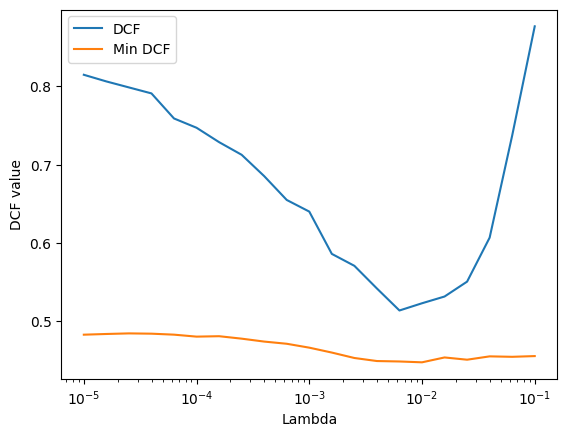
\includegraphics[width=\textwidth]{images/lr_lambda_100_prior.png}
        \caption{$\frac{1}{100}$ dataset}
        \label{fig:lr_lambda_100_prior}
    \end{subfigure}
    \caption{The figure shows the performance of LR models with prior-weighted models.}
\end{figure}

The new graphs show that same behavior of the previous ones. The regularization term is useful only when the number of samples is small. In general, the performance of the prior-weighted models is the same as the standard ones. This highlight the ability of logistic regression to handle different application setups.

\subsection{Expanded Feature Space}
The project investigates the performance of LR model as it varies the number of features used. The new features space is obtained by implementing polynomial expansion of the original features. The Figure \ref{fig:lr_lambda_quadratic} shows DCF and min DCF for different values of $\lambda$.

\begin{figure}[ht]
    \centering
    \begin{subfigure}[b]{0.45\textwidth}
        \centering
        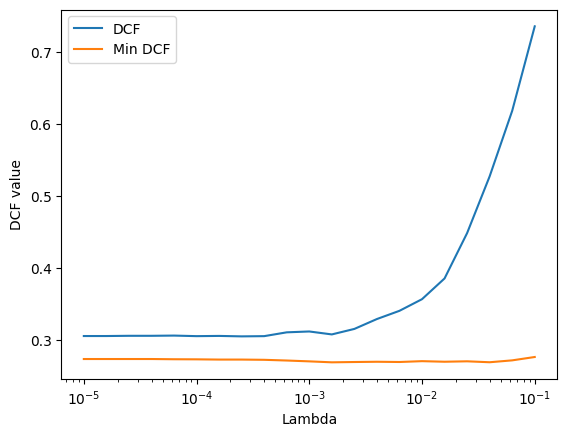
\includegraphics[width=\textwidth]{images/lr_lambda_quadratic.png}
        \caption{The figure shows the performance of LR models with expanded feature space.}
        \label{fig:lr_lambda_quadratic}
    \end{subfigure}
    \hfill
    \begin{subfigure}[b]{0.45\textwidth}
        \centering
        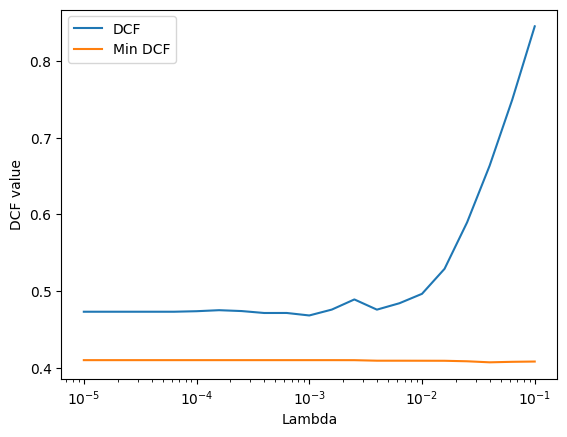
\includegraphics[width=\textwidth]{images/lr_lambda_centered.png}
        \caption{The figure shows the performance of LR models with centered features.}
        \label{fig:lr_lambda_centered}
    \end{subfigure}
\end{figure}

Both DCF and min DCF decrease quite a lot thanks to the new features. The regularization term has the same effect as before.

\subsection{Affine Transformation}
The project studies the performance of LR model with affine transformation of the features. In particular, the new features are centered versions of the original features. The Figure \ref{fig:lr_lambda_centered} shows the results.

The results show that the performance of the model is not affected particularly by the centered features.\\\\

Finally, after exploring different possible configuration, the best model is the one with the expanded feature space and $\lambda = 0.0015$ with min DCF equal to 0.269. LR models compared with MVG models perform better thanks to the expanded feature space that allows to capture the non-linear relationship between the features. This helps a lot explointing last two features that are grouped in clusters, so they are separable only with non-linear functions. Despite this MVG model is really good compared to LR linear model, in fact the min DCF are 0.308 and 0.407 respectively. This is due to the fact that the MVG model works really were when data matches the Gaussian distribution assumption.

\section{Lab 9: Support Vector Machines}
\label{sec:svm}
SVM is a powerful classification technique that finds the hyperplane that best separates the classes. The project investigates the performance of SVM model and its extension to non-linear cases. The experiments are conducted with k-fold cross-validation with k equal to 3, because the fitting procedure is very time consuming. The Figure \ref{fig:svm_C} shows the performance of SVM model as it varies the regularization parameter C evaluated with application setup (0.1, 1, 1).

\begin{figure}[ht]
    \centering
    \begin{subfigure}[b]{0.45\textwidth}
        \centering
        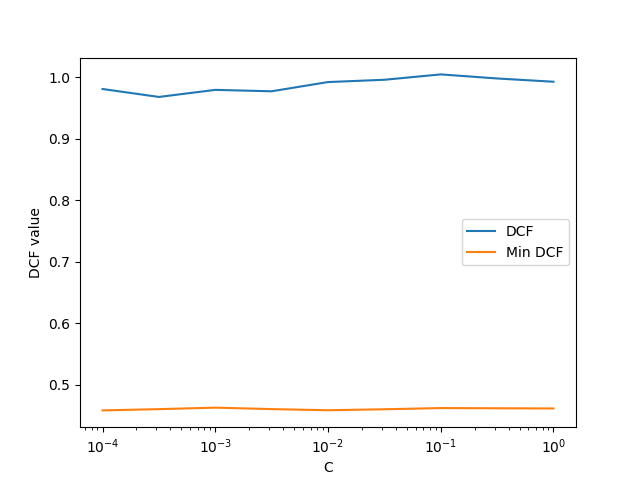
\includegraphics[width=\textwidth]{images/svm_C.png}
        \caption{The figure shows the performance of SVM models with different C.}
        \label{fig:svm_C}
    \end{subfigure}
    \hfill
    \begin{subfigure}[b]{0.45\textwidth}
        \centering
        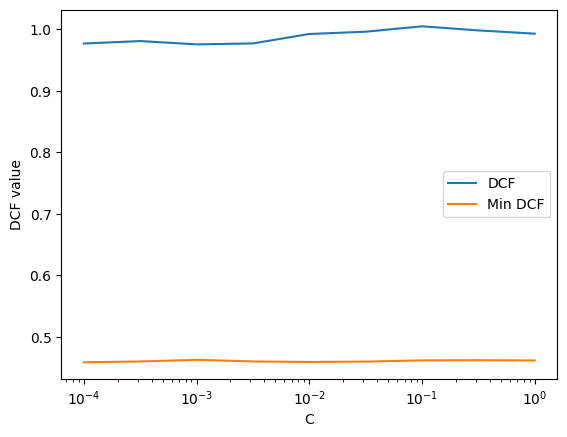
\includegraphics[width=\textwidth]{images/svm_C_centered.png}
        \caption{The figure shows the performance of SVM model with centered dataset.}
        \label{fig:svm_C_centered}
    \end{subfigure}
\end{figure}

The results show that the performance of the model is not affected by the regularization parameter C. DCF and min DCF are almost constant for all values of C. In every case, the actual DCF is pretty higher than min DCF, this means that the model is miscalibrated and it is not robust to application setup different from the empirical prior of the dataset. The linear SVM behaves worse than other linear models, in fact the min DCF is 0.458.

Further analysis are done using centered dataset to understand the difference respect to the standard one. The results shown in Figure \ref{fig:svm_C_centered} confirm the same behavior. There isn't any important difference between the two cases.

\subsection{Non-linear SVM}
The project considers two non-linear SVM models with polynomial and RBF kernels. The Figure \ref{fig:svm_C_poly} and Figure \ref{fig:svm_C_rbf} show the performance of SVM models with different C and RBF graph shows also different lines, one for each value of $\gamma$.

% \begin{figure}[ht]
%     \centering
%     \begin{subfigure}[b]{0.45\textwidth}
%         \centering
%         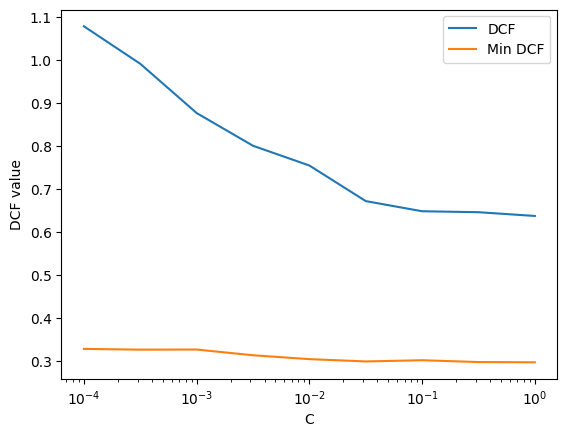
\includegraphics[width=\textwidth]{images/svm_C_poly.png}
%         \caption{The figure shows the performance of SVM models with polynomial kernel.}
%         \label{fig:svm_C_poly}
%     \end{subfigure}
%     \hfill
%     \begin{subfigure}[b]{0.45\textwidth}
%         \centering
%         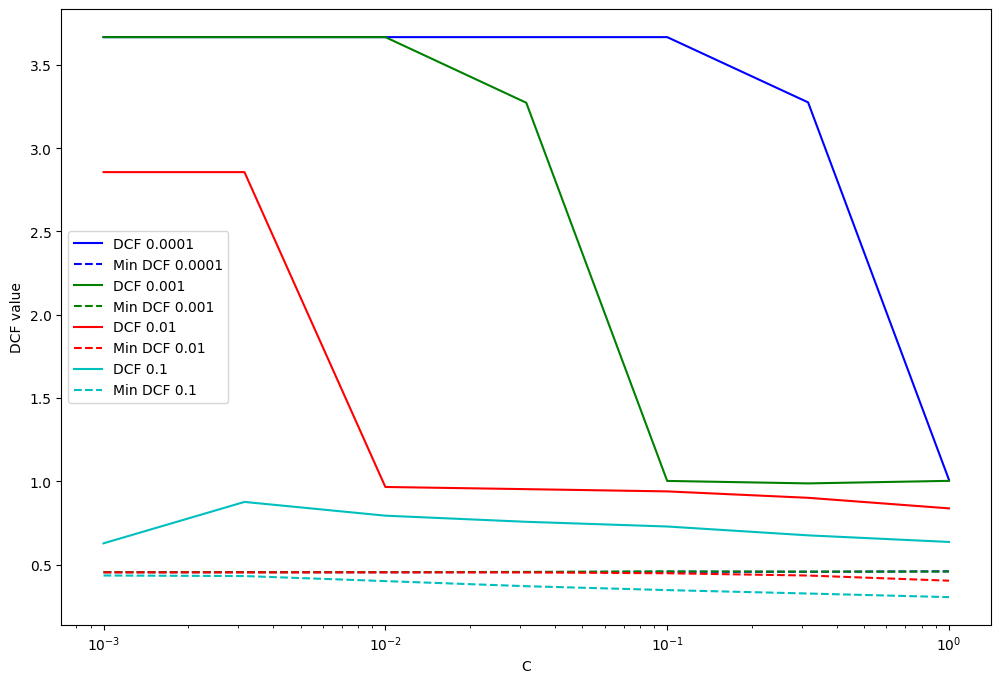
\includegraphics[width=\textwidth]{images/svm_C_rbf.png}
%         \caption{The figure shows the performance of SVM models with RBF kernel.}
%         \label{fig:svm_C_rbf}
%     \end{subfigure}
% \end{figure}

\section{Lab 10: Gaussian Mixture Models}
\label{sec:gmm}
Finally, as the last model, the project investigates the performance of Gaussian Mixture Models (GMM). The experiments are conducted with k-fold cross-validation with k equal to 10. The Figure \ref{fig:gmm_M} shows the performance of GMM models as it varies the number of components M and the covariance matrix.

\begin{figure}[ht]
    \centering
    \begin{subfigure}[b]{0.45\textwidth}
        \centering
        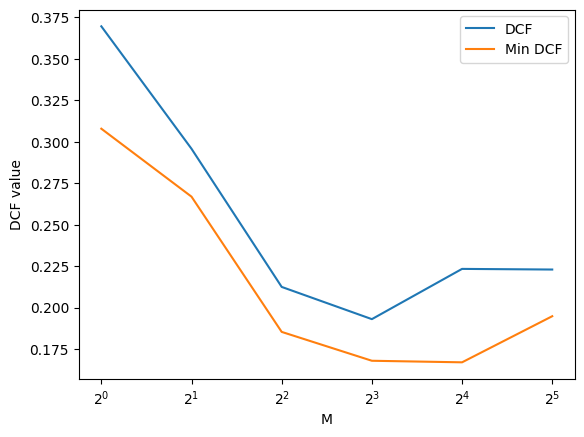
\includegraphics[width=\textwidth]{images/gmm_M.png}
        \caption{GMM model}
    \end{subfigure}
    \hfill
    \begin{subfigure}[b]{0.45\textwidth}
        \centering
        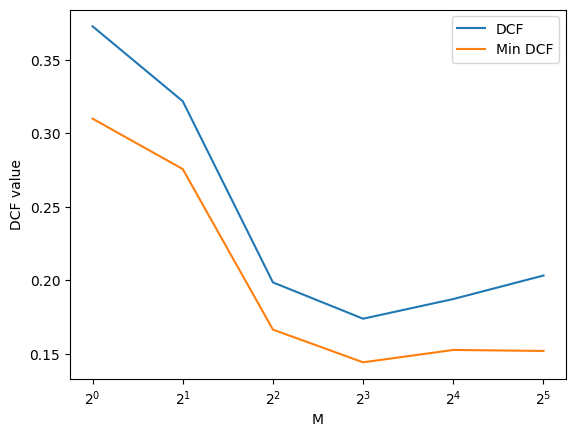
\includegraphics[width=\textwidth]{images/gmm_M_diagonal.png}
        \caption{Diagonal GMM model}
    \end{subfigure}
    \caption{The figure shows the performance of GMM models with different M and covariance matrix.}
    \label{fig:gmm_M}
\end{figure}

\begin{figure}[ht]
    \centering
    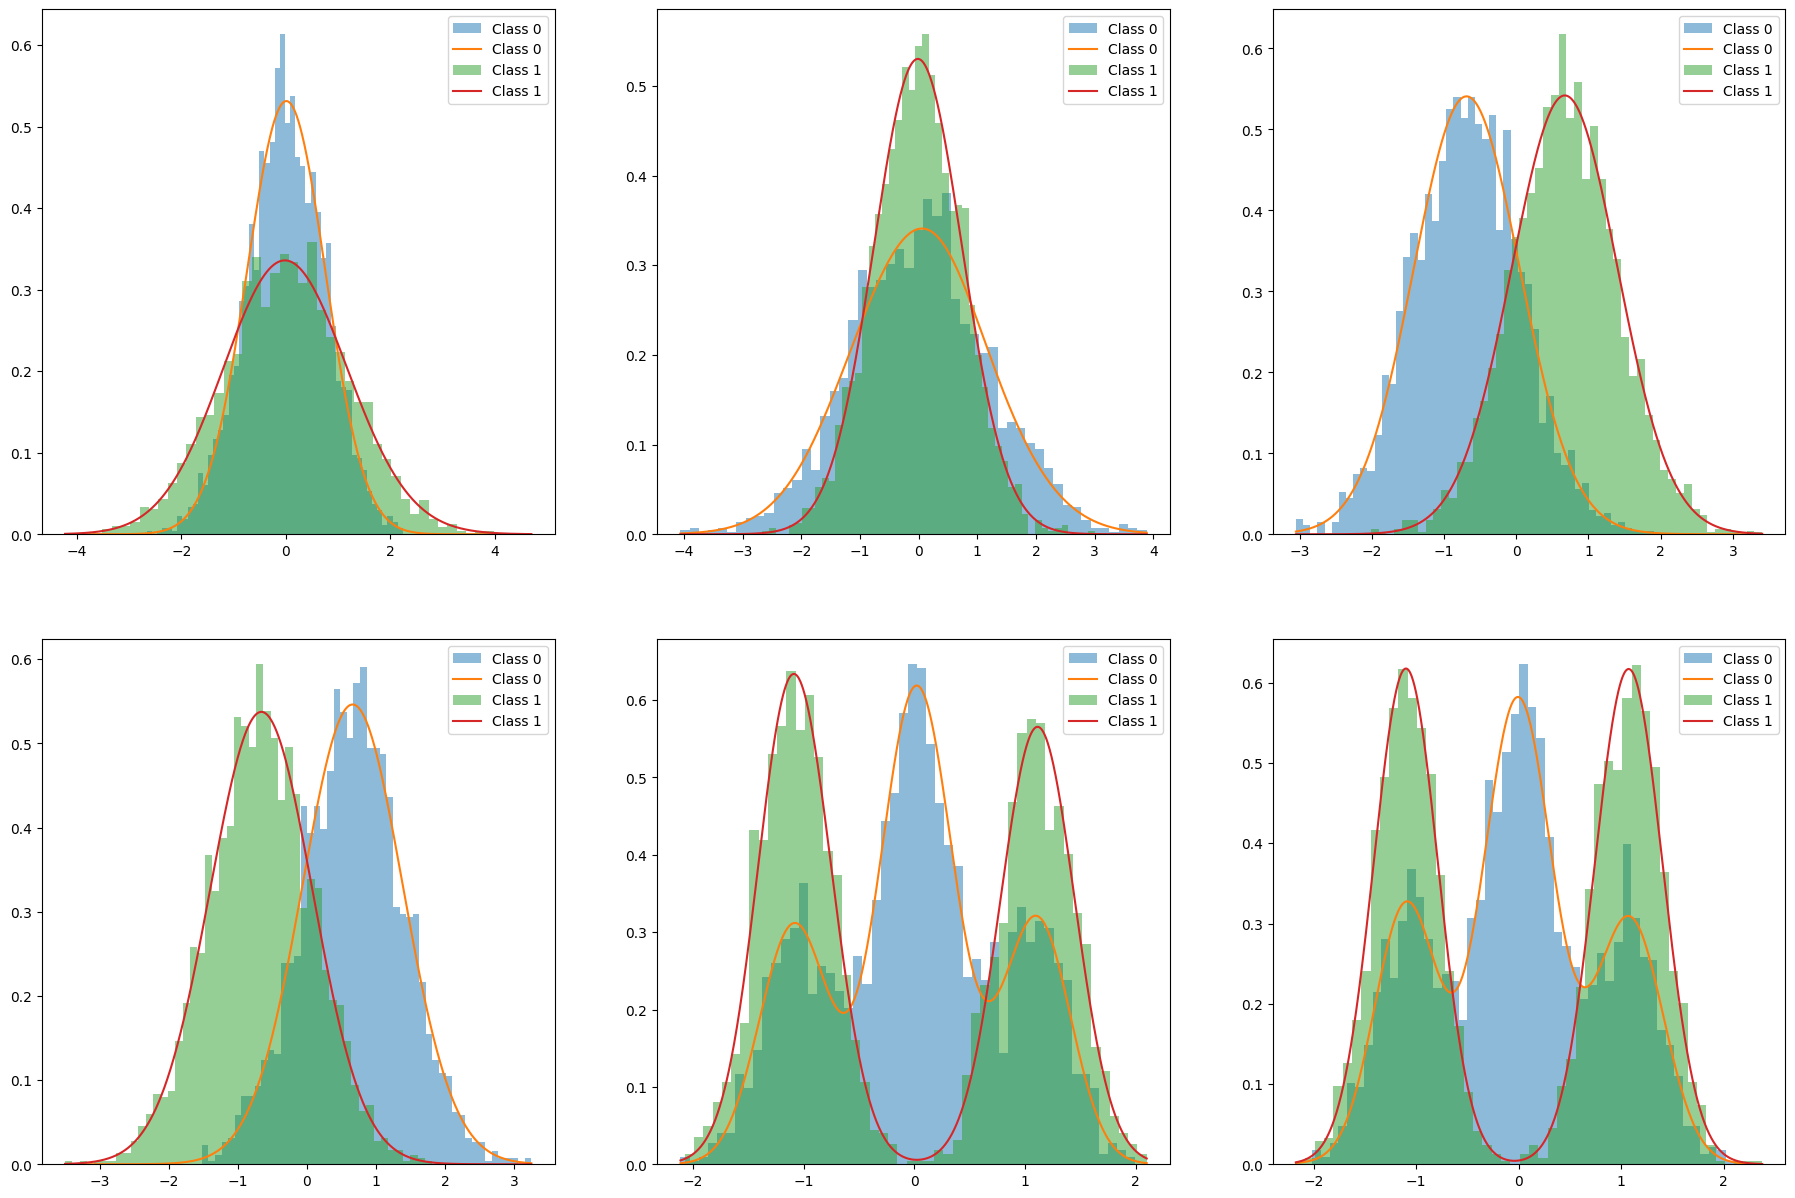
\includegraphics[width=\textwidth]{images/dataset_gmm.png}
    \caption{The figure shows the histograms of the dataset and the Gaussian Mixture Model that best fits the data.}
    \label{fig:dataset_gmm}
\end{figure}

The results of Tied GMM are not presented as they are bad as always, the assumptions done are not compatible with the dataset. Surprisingly, the Diagonal GMM model performs better than the standard one. The Min DCF is the lowest of the project and it is equal to 0.144 with 8 components. To further analyze the reason behind the Figures \ref{fig:dataset_gmm} and \ref{fig:dataset_gmm_diagonal} compare the distribution of the data with the multimodal Gaussian density function estimated by the models.

\begin{figure}[ht]
    \centering
    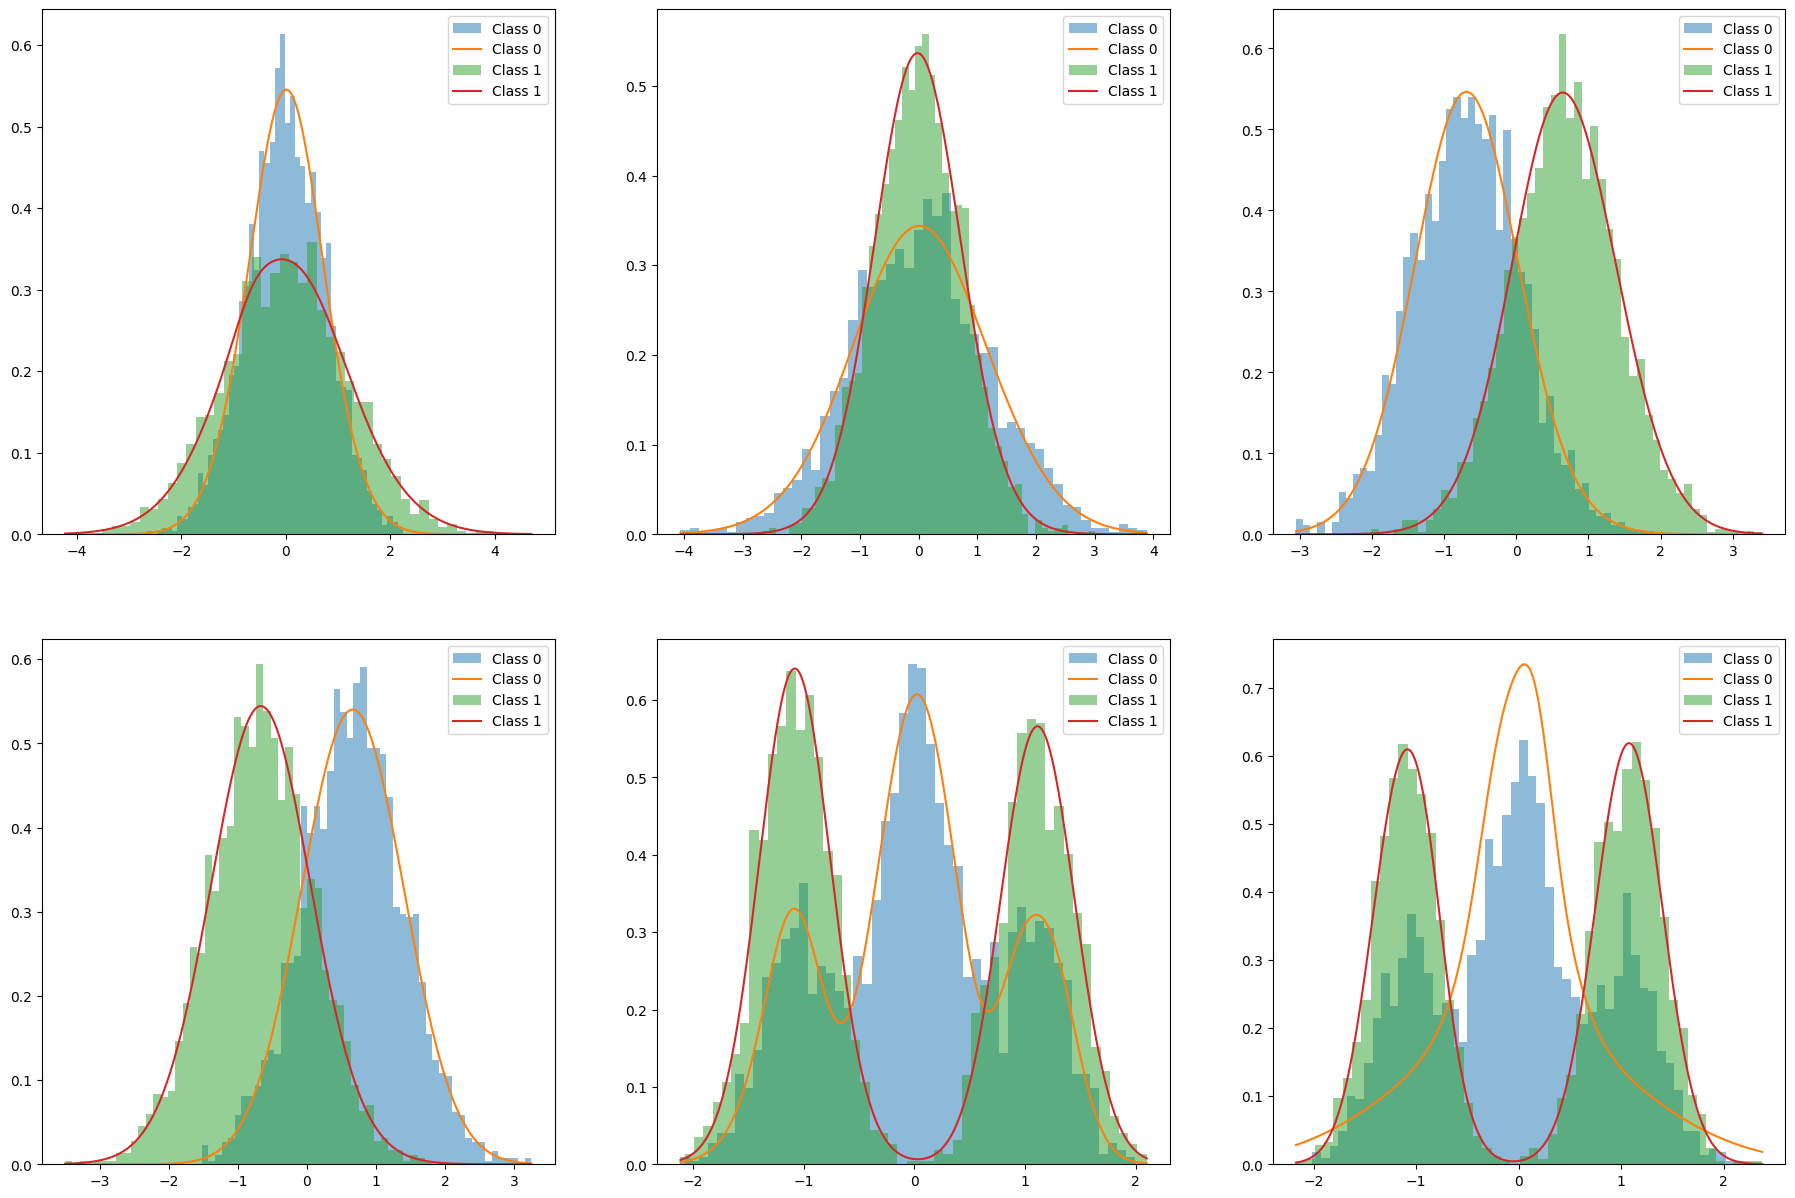
\includegraphics[width=\textwidth]{images/dataset_gmm_diagonal.png}
    \caption{The figure shows the histograms of the dataset and the Diagonal Gaussian Mixture Model that best fits the data.}
    \label{fig:dataset_gmm_diagonal}
\end{figure}

The only significative difference between the two models is on the features 6, where diagonal model presents a unimodal Gaussian density function, while the standard model presents a trimodal one. 

\section{Lab 11: Calibration}

\subsection{Model comparison}
Before the calibration, the project compares the performance of the best models for each technique. Particularly, they are compared on Bayes Error plot. The Table \ref{tab:models_performance} makes a summary of the performance of the best models seen until now with application setup (0.1, 1, 1) and k-fold with k equal to 3. The Figure \ref{fig:models_bayes_error} shows the actual DCF and min DCF for different application priors.

\begin{table}[ht]
    \centering
    \begin{tabularx}{\textwidth}{lXXX}
        \toprule
        \textbf{Model} & \textbf{DCF} & \textbf{Min DCF} \\
        \midrule
        LR & 0.321 & 0.3 \\
        SVM & - & - \\
        GMM & 0.185 & 0.157 \\
        \bottomrule
    \end{tabularx}
    \caption{Performance metrics for the best models with application setup (0.1, 1, 1).}
    \label{tab:models_performance}
\end{table}

The configuration parameters for each model are:
\begin{itemize}
    \item LR: expanded feature space and $\lambda = 0.0015$.
    \item SVM: Polynomial kernel with degree 4 and c equal to 1.
    \item GMM: 8 components and full covariance matrix.
\end{itemize}

\begin{figure}[ht]
    \centering
    \begin{subfigure}[b]{0.3\textwidth}
        \centering
        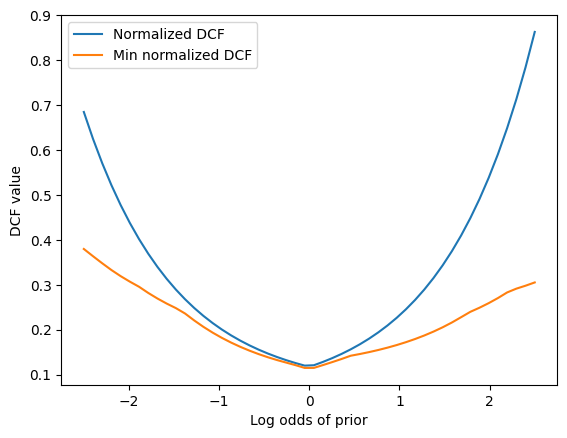
\includegraphics[width=\textwidth]{images/lr_bayes_error.png}
        \caption{LR.}
    \end{subfigure}
    \hfill
    % \begin{subfigure}[b]{0.3\textwidth}
    %     \centering
    %     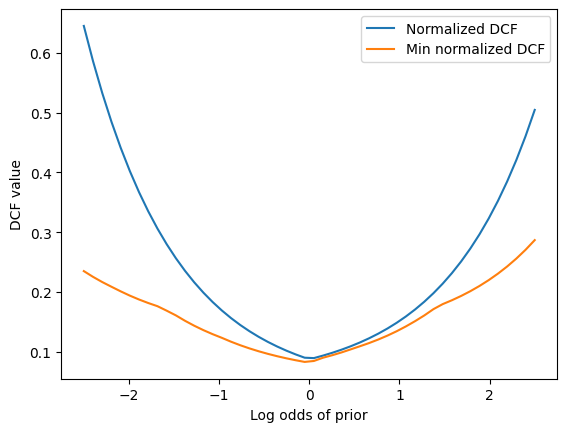
\includegraphics[width=\textwidth]{images/svm_bayes_error.png}
    %     \caption{SVM.}
    % \end{subfigure}
    \hfill
    \begin{subfigure}[b]{0.3\textwidth}
        \centering
        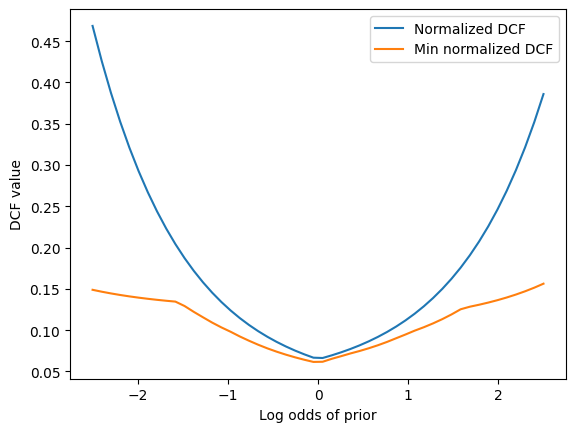
\includegraphics[width=\textwidth]{images/gmm_bayes_error.png}
        \caption{GMM.}
    \end{subfigure}
    \caption{The figure shows the Bayes error plot for the best models with application setup (0.1, 1, 1).}
    \label{fig:models_bayes_error}
\end{figure}


\end{document}
